\documentclass[12pt]{article}
\usepackage{jcappub}
\usepackage{amsmath}
\usepackage{graphicx}
\usepackage{mathtools} %For summations with limits
\usepackage{multicol} %For multiple columns
\setlength{\columnsep}{1cm}


\title{The Distribution of Vacua in Random Landscape Potentials}

\author{Low Lerh Feng,}
\author{Shaun Hotchkiss}
\author{and Richard Easther}

\emailAdd{lerh.low@auckland.ac.nz}
\emailAdd{s.hotchkiss@auckland.ac.nz}
\emailAdd{r.easther@auckland.ac.nz}

\newcommand{\re}[1]{\textcolor{blue}{[{\bf RE}: #1]}}
\newcommand{\lfl}[1]{\textcolor{red}{[{\bf LL}: #1]}}


\affiliation{Department of Physics,\\ University of Auckland, \\Private Bag 92019,\\ Auckland, New Zealand}



\abstract{
We analyze the distribution of stationary points of multi-dimensional random Gaussian fields of known field value. We find an analytical expression for this distribution, from which we calculate the probability that a given maximum has a field value below the average, or equivalently a given minimum has a field value above the average. The complexity of the expression increases very quickly with the number of dimensions. We present analytic results up until 6 dimensions, and numerical results to 10 dimensions. Although our motivations stem from cosmology, the results depend only on the properties of random Gaussian fields.}

\begin{document}



\maketitle

\section{Introduction}

\re{We should start this with a discussion of the multiverse / landscape and the anthropic selection of the vacuum energy; our main point is about $P(\Lambda)$ not inflation, and be clear about the difference between a random potential and {\em the} string landscape. I am probably best placed to do this} 

The theory of inflation is the current best explanation for certain perplexing observations of the Universe, such as the monopole problem, horizon problem, and flatness problem. Inflation is thought to be caused by a scalar field, but the exact nature of this field is shrouded in unknowns. The simplest possibility is a one-dimensional scalar field analogous to the gravitational potential; however multidimensional scalar fields are also possible. In particular, string theory predicts the existence of a highly complex, $O(100)$ dimensional scalar field known as the \emph{landscape}. The string landscape is so complex that quantitative predictions are hard to extract; as a result, most studies of the landscape assume it is a Gaussian random field.\cite{GRF1, GRF2, GRF3} Physically, this assumption works if the individual terms that make up the landscape are sufficiently uncorrelated that the central limit theorem is applicable.

An early study using this assumption was by Aazami and Easther \cite{Aazami2006}, which took the Hessian of a random function to be symmetric matrices with random individual elements, or more precisely, with values randomly drawn from a Gaussian distribution (called a Gaussian Orthogonal Ensemble [GOE]). From elementary calculus, a minimum exists if the eigenvalues of the Hessian are all positive, a maximum exists if they are all negative, and there is a saddle if there are eigenvalues of both signs. Using the GOE, they find that the number of minima is super-exponentially small compared to the number of saddles. This approach was later shown to be incorrect, because the eigenvalues of the Hessian of a random function are not independent of each other \cite{Easther2016}. Taking this into account, the authors found that the number of minima decreases exponentially with the number of dimensions $N$ instead, and the ratio of extrema to saddles to be approximately binomial.

In addition to the probability of minima, the distribution of eigenvalues of the Hessian about minima as well as the distribution of the Hessian itself as a function of $N$ has also been investigated.\cite{Yamada2018} Yamada and Vilenkin found that in a Gaussian random landscape the smallest eigenvalue is of order $\sim 1/N$, which, if one assumes that the most probable decay pathway is in the direction of the smallest eigenvalues, improves the stability of the minima by about $\sqrt{N}$.

In all these works, the statistics of stationary points at a given field value has not been studied. In standard inflation theory, the universe inflates when the gradient of the potential is small (so-called ``slow-roll inflation"), and stops inflating when we reach the potential's minimum. If the minimum is a global minimum, then the end state is stable. If it is only a local minimum, then in principle the universe might quantum tunnel to an even lower-potential state, but it is usually assumed in landscape models that the local minimum is metastable, with a lifetime much greater than the age of the universe. Nonetheless, if the local minimum has a value above zero, then this can manifest as a nonzero dark energy term. Therefore, the probability a minima has potential value above zero is a desirable number to know. This probability is investigated in our paper. We will begin with an overview of the theory, followed by analytical results and numerical results up to $N=10$. We will then discuss some general features of this probability, and finally present our conclusions.

\section{Theory}

\re{This needs to start ``further back'' -- we don't want to recap all of BBKS, but we need to define what a random function is, dimensionality, the connection between that  and the potential we associate with the landscape, and walk people through the Kac-Moody formula so they can see why we're doing what we're doing. It does not need to be a book, but I would imagine it as a couple of pages, and also to be clear about the difference between paper and the one I had with Guth and Masoumi}

Our analysis is an N-dimensional generalization of Appendix A in Bardeen, Bond, Kaiser and Szalay (henceforth BBKS) \cite{BBKS}. We adopt ths same notation, $\eta_i \equiv \frac{\partial \phi}{\partial x^i}, \xi_{ij} \equiv \frac{\partial^2 \phi}{\partial x^i \partial x^j}$. In this notation, the correlations of a Gaussian random field at a random point in N-dimensions are:

\begin{equation} \label{corr}
\begin{split}
\langle\phi\phi\rangle &= \sigma_0^2 \\
\langle\eta_i\eta_j\rangle &= \frac{1}{N}\delta_{ij}\sigma_1^2 \\
\langle\phi\eta_{ij}\rangle &= -\frac{1}{N}\delta_{ij}\sigma_1^2 \\
\langle\xi_{ij}\xi_{kl}\rangle &= \frac{1}{N(N+2)}\sigma_2^2(\delta_{ij}\delta_{kl}+\delta_{il}\delta_{jk}+\delta_{ik}\delta_{jl})
\end{split}
\end{equation}

\noindent Here $\phi$ indicates the field value, and the $\sigma$'s are the moments of the power spectrum. For $N=3$ this reduces to BBKS's equation A1. We define the following vector:

\begin{equation}
\begin{split}
\alpha_i = \{\phi,\eta_1,\eta_2,\ldots,\xi_{11},\xi_{22},\ldots,\xi_{NN},\xi_{N-1,N},\xi_{N-2,N},\ldots,\xi_{1N},\xi_{N-2,N-1},\\
\ldots\xi_{1,N-1},\ldots,\xi_{12}\}
\end{split}
\end{equation}

\noindent The subscript $i$ serves only as an identifier for the element of the vector (e.g. $\alpha_1 = \phi$) and has no other meaning. We define the covariance matrix $M_{ij}\equiv\langle\alpha_i\alpha_j\rangle$ and its inverse $K \equiv M^{-1}$. Working through the math, one can see that given the correlations in Eq. \ref{corr}, the correlation matrix is not diagonal, for example in 3 dimensions it takes the following form: \re{Can we write down the general form; possibly as a block matrix with the individual blocks show separate -- better to avoid giving examples for specific $N$; we have used the examples as ``handholds'' as we figure this out }

\[
M=
  \begin{bmatrix}
    \sigma_0^2 & 0 & 0 & 0 & -\frac{\sigma_1^2}{3} &  -\frac{\sigma_1^2}{3} & -\frac{\sigma_1^2}{3} & 0 & 0 & 0\\
    0 & \frac{\sigma_1^2}{3} & 0 & 0 & 0 & 0 & 0 & 0 & 0 & 0\\
    0 & 0 & \frac{\sigma_1^2}{3} & 0 & 0 & 0 & 0 & 0 & 0 & 0\\
    0 & 0 & 0 & \frac{\sigma_1^2}{3} & 0 & 0 & 0 & 0 & 0 & 0\\
    -\frac{\sigma_1^2}{3} & 0 & 0 & 0 & \frac{\sigma_2^2}{5} & \frac{\sigma_2^2}{15} & \frac{\sigma_2^2}{15} & 0 & 0 & 0\\
    -\frac{\sigma_1^2}{3} & 0 & 0 & 0 & \frac{\sigma_2^2}{15} & \frac{\sigma_2^2}{5} & \frac{\sigma_2^2}{15} & 0 & 0 & 0\\
    -\frac{\sigma_1^2}{3} & 0 & 0 & 0 & \frac{\sigma_2^2}{15} & \frac{\sigma_2^2}{15} & \frac{\sigma_2^2}{5} & 0 & 0 & 0\\
    0 & 0 & 0 & 0 & 0 & 0 & 0 & \frac{\sigma_2^2}{15} & 0 & 0\\
    0 & 0 & 0 & 0 & 0 & 0 & 0 & 0 & \frac{\sigma_2^2}{15} & 0\\
    0 & 0 & 0 & 0 & 0 & 0 & 0 & 0 & 0 & \frac{\sigma_2^2}{15}\\
  \end{bmatrix}
\]

The probability distribution of $\alpha$ is (by definition for Gaussian random fields \re{this is something you derive, not something you define -- we should sketch how this works})

\begin{equation} \label{ProbDistrib}
p(\alpha_i)=\frac{1}{(2\pi)^{N(N+3)/4}\sqrt{\mathrm{det}M}} e^{-\frac{1}{2}\alpha K \alpha}
\end{equation}

For the purpose of this paper, the only term that matters is the exponential. This is because the coefficient is a constant, we are interested in the probability that a minimum has field value above zero, i.e. $p(\phi>0)/p(-\infty<\phi<\infty)$, and in a ratio all the constant factors cancel.

Like BBKS, we transform to a different basis; however the basis we choose is different from BBKS:

\begin{align*}
\begin{split}
\sigma_2x = -\nabla^2\phi &= -(\xi_{11}+\xi_{22}+\ldots+\xi_{NN})\\
\sigma_2y &= -(\xi_{11}-\xi_{22})\\
\sigma_2z &= -(\xi_{11}+\xi_{22}-\xi_{33})\\
\sigma_2a &= -(\xi_{11}+\xi_{22}+\xi_{33}-\xi_{44})\\
\ldots
\end{split}
\end{align*}

We pick this basis because it simplifies the integration region later in the analysis, which we find gives the fastest computational time; however in principle all bases should give the same result. Following BBKS, we introduce $\nu = F/\sigma_0$. With this choice of basis, the nonzero correlations are \re{maybe say why, at least for an exampke}:

\begin{gather}
\langle\nu^2\rangle = 1, \langle x^2\rangle=1, \langle y^2 \rangle = \langle \xi_{11}^2 -2\xi_{11}\xi_{22} + \xi_{11}^2\rangle = \frac{4}{N(N+2)} \\
\langle z^2 \rangle = \frac{12}{N(N+2)}, etc.
\end{gather}

From here, the factor $\alpha K \alpha$ ($Q$ in BBKS) in Eq. \ref{ProbDistrib} takes the form

\begin{equation} \label{Q}
\begin{split}
2Q = \nu^2 + \frac{(x-x_*)^2}{1-\gamma^2} + \frac{N(N+2)}{4}y^2 + \frac{N(N+2)}{12}z^2 + \ldots + \frac{N \pmb{\eta}\cdot \pmb{\eta}}{\sigma_1^2} \\
+ \sum_{i,j;i > j}^N\frac{N(N+2)\xi_{ij}}{\sigma_2^2}
\end{split}
\end{equation}

\noindent where $x_* \equiv \gamma x$ and $\gamma = \frac{\sigma_1^2}{\sigma_2 \sigma_0}$. This is the equivalent of BBKS Eq. (A4) for N-dimensions. Note the first two terms remain constant for all $N$, but the remaining terms vary. The $\eta$ terms are zero at minima by definition, while the off-diagonal $\xi_{ij}$ terms can be Euler-rotated away by choosing an appropriate set of axes. The $\xi$ matrix is already symmetric (by rotational symmetry), and Euler rotation turns it diagonal.\cite{Goldstein} The upshot is that the symmetric $\xi$ matrix becomes a diagonal matrix where the individual elements are the eigenvalues $\lambda_i = -\xi_{ii}$ of the Hessian. We are interested in minima, hence we demand all second derivatives to be positive, i.e. all eigenvalues to be negative. From here, the analysis is exactly the same as BBKS, except that when we define the ordering of the eigenvalues $\lambda_1 \geq \lambda_2 \geq \lambda_3 \ldots \geq 0$, our boundary conditions are significantly simpler because of the different choice of basis. For example, in 3D, our conditions are $y \geq 0, y \leq z$, and $x \geq z$ (compare BBKS's equation between Eq. (A14) and Eq. (A15)).

The final expression we arrive at for the density of peaks is:

\begin{equation} \label{DensityOfPeaks}
N = A \int_{\lambda_1 \geq \lambda_2 \geq \lambda_3 \ldots \geq 0} F \times e^{-Q} d\nu dx dy dz \ldots
\end{equation}

\noindent where

\begin{equation}
F = \lambda_1\lambda_2\lambda_3\ldots\lambda_N \sum^N_{i,j; i>j} (\lambda_i - \lambda_j),
\end{equation}

\noindent $Q$ is given by Eq. \ref{Q}, $A$ is some constant factor, and the integration limits are only over the region where the conditions are satisfied. 

\section{Peak numbers as a function of height}

\re{I think we want to develop the general problem of finding the number of peaks/minima as a function of $V$; we can develop both via the Monte Carlo integrals and via the ``peak ratio'' method, and perhaps even showing examples for specific realisations for $N$ from 2 to 5.  We could do this as a set of subsections.}  

In principle, evaluating the $x, y, z \ldots$ integrals leaves just a $\nu$ integral, and the desired probability is the integral over $0 \leq \nu \leq \infty$ divided by the integral over $-\infty \leq \nu \leq \infty$. In practice, the complexity of the integral rises quickly. Although the result in 3D contains only a few terms (c.f. BBKS Eq. (A15)), the 4D integral has 14 terms, and the 5D integral over eight hundred (our tool of choice, Mathematica, even fails to analytically integrate the 5D result unless a different basis is used).


The final probability depends not only on the field value $\phi$ but also the moments of the power spectrum $\sigma_0, \sigma_1, \sigma_2$. However, it turns out that two of the three $\sigma$'s are normalizable. $\sigma_0$ is closely related to the average value of the field (see Eq. \ref{corr}), so with an appropriate choice of the zero of the field, we can set $\sigma_0 = 1$. Similarly, $\sigma_1$ represents the average of the first derivatives, and with an appropriate rescaling of the axis length we can also set it $\sigma_1 = 1$. This leaves $\sigma_2$ as the only remaining parameter, and all the results we present will be in terms of $\sigma_2$.

\begin{figure}
  \centering
  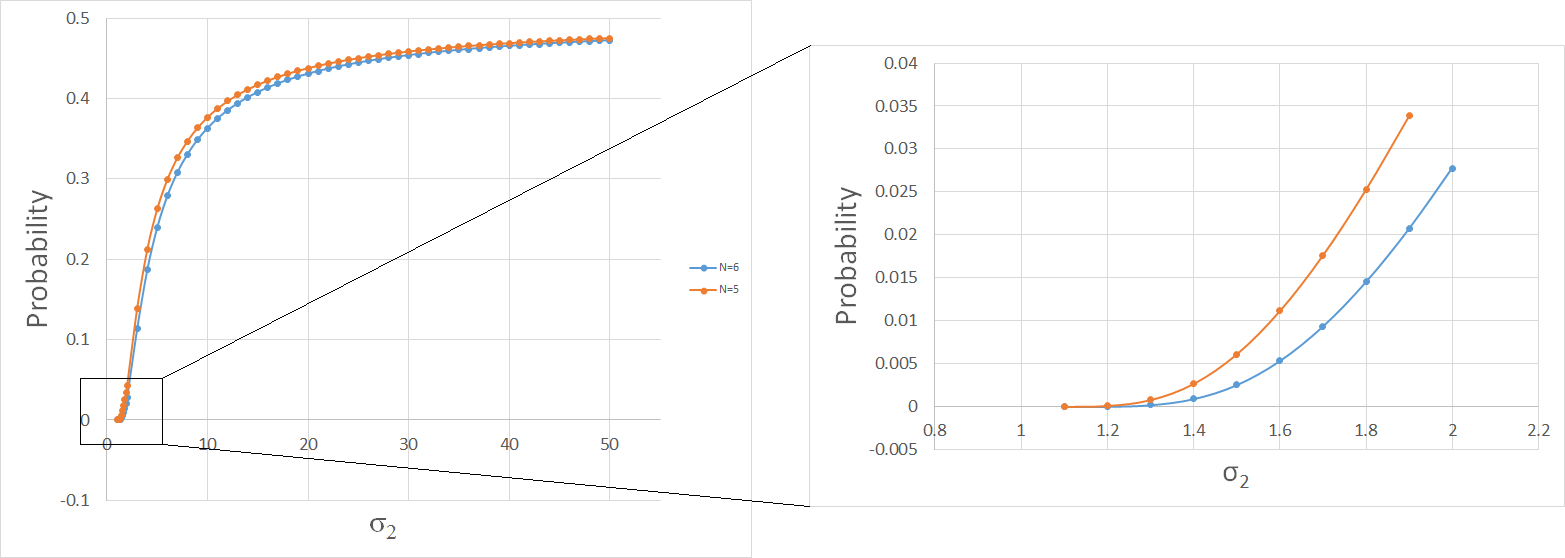
\includegraphics[width=\linewidth]{N6minima.png}
  \caption{The probability that a given extremum with $\phi > 0$ is a minimum as a function of $\sigma_2$, for $N=5,6$. A close-up of the probabilities for small values of $\sigma_2$ is shown as well. The probability for $N=5$ is always larger than that for $N=6$.}
  \label{N6}
\end{figure}

In Fig. \ref{N6}, we present the probability that a given extremum with $\phi > 0$ is a minimum as a function of $\sigma_2$. As expected, if the potential is highly oscillatory (i.e. $\sigma_2$ is large, or $\gamma$ is small), the probability tends towards 0.5 -- equal likelihood of an extremum being either a maximum or a minimum. Conversely, if the potential is very smooth ($\sigma_2$ is small), the probability tends towards 0. Further, for any given $\sigma_2$, the probability decreases with increasing dimension.

For $N > 6$, the integral is complex enough that Mathematica struggles to get analytical results. To make further progress, we have written a C++ code to perform the numerical integration, using the VEGAS \cite{VEGAS} monte carlo integration routines of the GNU Scientific Library.\cite{GSL} The code is only able to perform the integral for a given value of $\phi$ and $\gamma$. However, with enough data points, it becomes possible to numerically evaluate the probability using the trapezoidal rule. Using $\phi$ in steps of 0.5, we confirm that the numerical integration code matches the analytical integration for $N < 6$ to two digits of precision; we also confirm that agreement improves if we increase the resolution of $\phi$. For example, for $N=4, \sigma_2=3.5$, the exact probability is 0.21005. Comparatively, integrating with the trapezoidal rule with $\phi$ in steps of 0.5 gives a probability of 0.215202; with $\phi$ in steps of 0.1, this changes to 0.210256. This gives us confidence in the numerical results for $N > 6$. We present some data up until $N = 10$ in Table 1; beyond $N = 10$, even the numerical integration fails to produce results.

\begin{table}[h!]
  \begin{center}
    \caption{The probability that a given extremum with $\phi > 0$ is a minimum as a function of $\sigma_2$. Values given for $N=4,5,6$ are exact; for larger values they are approximate (see the text; errors are on the order of the third nonzero digit after the decimal).}
    \label{tab:table1}
    \begin{tabular}{c|c|c} % <-- Alignments: center/center/center (l and r for left and right if needed)
      $\textbf{N}$ & $\sigma_2$ & $p_{min}$\\
      \hline
      4 & 10 & 0.60859\\
      5 & 10 & 0.62333\\
      6 & 10 & 0.63680\\
      7 & 10 & 0.35210\\
      8 & 10 & 0.34227\\
      9 & 10 & 0.33159\\
      10 & 10 & 0.32151\\
      \hline
      4 & 3.5 & 0.21520\\
      5 & 3.5 & 0.17886\\
      6 & 3.5 & 0.15274\\
      7 & 3.5 & 0.13599\\
      8 & 3.5 & 0.11711\\
      9 & 3.5 & 0.10093\\
      10 & 3.5 & 0.08729\\
      \end{tabular}
      \quad
      \begin{tabular}{c|c|c} 
      $\textbf{N}$ & $\sigma_2$ & $p_{min}$\\
      \hline
      4 & 2 & 0.066638\\
      5 & 2 & 0.043103\\
      6 & 2 & 0.030844\\
      7 & 2 & 0.02013\\
      8 & 2 & 0.01307\\
      9 & 2 & 0.00845\\
      10 & 2 & 0.00544\\
      \hline
      4 & 1.25 & 0.001526\\
      5 & 1.25 & 0.000327\\
      6 & 1.25 & 6.53328 $\times 10^{-5}$\\
      7 & 1.25 & 2.09673 $\times 10^{-5}$ \\
      8 & 1.25 & 3.97235  $\times 10^{-6}$ \\
      9 & 1.25 & 7.13489  $\times 10^{-7}$ \\
      10 & 1.25 & 1.20253  $\times 10^{-7}$ \\
     \end{tabular}
  \end{center}
\end{table}

\begin{figure} 
  \centering
  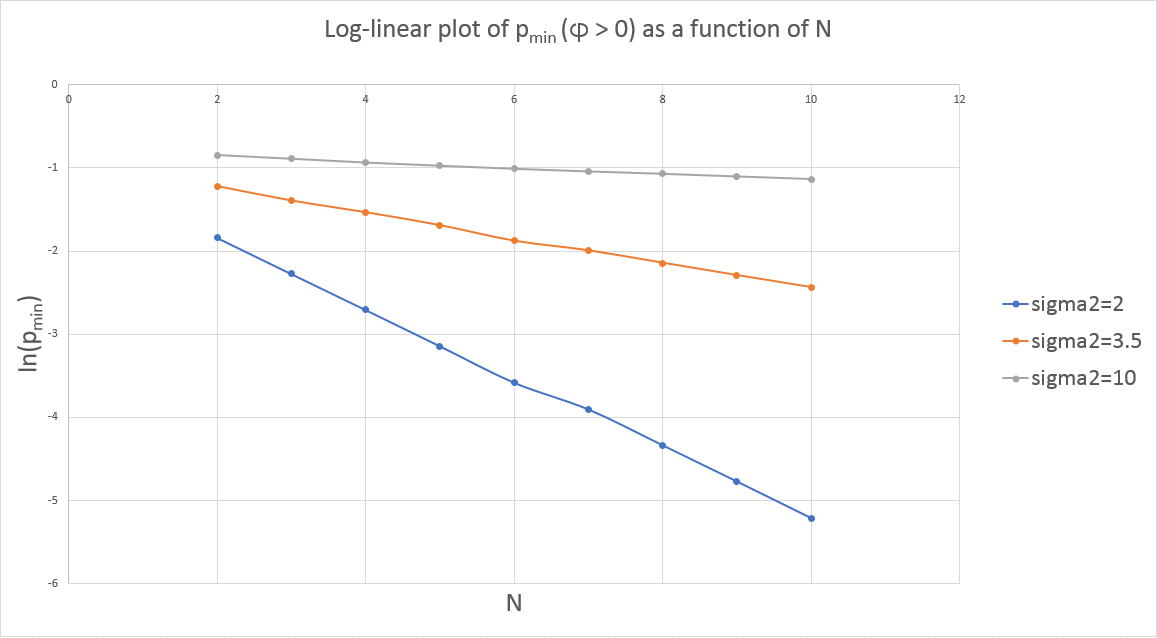
\includegraphics[width=\linewidth]{Log-linear.png}
  \caption{A log-linear plot of the probability that a given extremum with $\phi > 0$ is a minimum for a given $\sigma_2$, as a function of the number of dimensions $N$.}
  \label{Log-Linear}
\end{figure}

\section{Implications for Multiverse Cosmology}

\re{I would move from looking at the abstract problem in the previous section to the specific implications for cosmology in this section; and how $P(\Lambda)$ depends on $\sigma_2$}

As can be seen, the probability that a given extremum with $\phi > 0$ is a minimum decreases with increasing $N$. For a constant $\sigma_0$ and $\sigma_1$, the probability also decreases for increasing $\sigma_2$. Both of these general trends are to be expected: as $N$ increases, there are more conditions that must be simultaneously met for a point to be a minimum, hence the probability decreases. Also, since $\sigma_2$ is the average of the second derivative of the field, as $\sigma_2$ increases the field gets more and more turbulent. This means there are both more maxima and more minima, and the probability decreases.

In Fig. \ref{Log-Linear}, we present a log-linear plot of the probability against the dimension for the three values of $\sigma_2$. The resulting lines are surprisingly straight. There is a noticeable kink in both the $\sigma_2 = 3.5$ and $\sigma_2=2$ case between $N=6$ and $N=7$. This is a numerical effect -- it is where the exact results end and the numerical ones begin. We checked this by running the numerical integration for $N=6$ as well. Replacing the exact result with the numerical one, the kink moves to the left. The kink indicates that the numerical results are consistently overestimating the true probability, but that is not surprising because the numerical results rely on the trapezoidal rule. The trapezoidal rule overestimates the result when the integral is concave up, and underestimates it when it is concave down. The final probability is the area under the curve for $\phi > 0$ divided by the area under the curve for all $\phi$. From Fig. \ref{Likelihood}, for $\phi > 0$ the curve is concave up, so the trapezoidal rule overestimates the numerator, and accordingly the probability as well. This trend holds for higher $N$ as well, since in for higher $N$ the plot moves to more negative values.

\begin{figure}
  \centering
  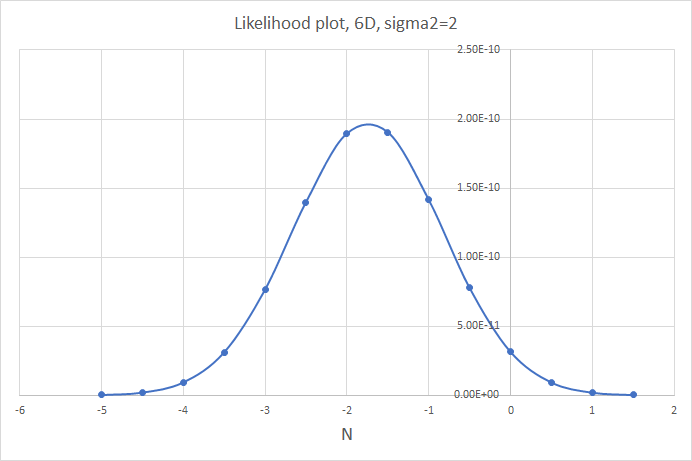
\includegraphics[width=\linewidth]{LikelihoodPlot.png}
  \caption{A plot of the likelihood for $\sigma_2=2, N=6$. The final probability desired is the area under the curve for $\phi > 0$ divided by the area unde the curve for all $\phi$. For the region $\phi > 0$, the curve is concave upwards, so the trapezoidal rule overestimates its value. Accordingly, the numerator and probability are also overestimated.}
  \label{Likelihood}
\end{figure}

If the trend is robust, then for the case of $\sigma_2=2$, the probability at $N=100$ is of the order of $p \sim 10^{-42}$. Since there are $\sim 10^{500}$ stationary points in the landscape,\cite{Douglas} this probability, while small, still leads to there being $\sim 10^{458}$ minima that might correspond to our universe.

\section{Conclusion}
We have presented results for the statistics of stationary points at a given field value as a function of $N$ and $\sigma_2$. The numbers confirm the intuitive expectation that the probability of a given extremum with $\phi > 0$ being a minimum decreases as $N$ increases or when $\sigma_2$ decreases. We also present a first estimate for the probability at $N=100$ for the $\sigma_2=2$ case, $p \sim 10^{-42}$. However, reliable results are only available up to $N=10$. To push these results up to even greater $N$ is the next goal.

\section{Appendix}
For $N=4$, the full form of the integral Eq. \ref{DensityOfPeaks} is:

\begin{equation}
\begin{split}
N = \frac{1}{214990848} \mathrm{Exp}\frac{9x^2\sigma_1^4 + 2\nu x \sigma_0 \sigma_1^2 \sigma_2 - (v^2+10x^2)\sigma_0^2\sigma_2^2}{-2\sigma_1^4+2\sigma_0^2\sigma_2^2}\\\bigg{(}80x - 1610e^{3x^2}+128x^3+418e^{3x^2}x^3+4e^{4x^2}\sqrt{\pi}(3+48x^2+64x^4)\mathrm{Erf}[\sqrt{\frac{3}{2}}x]\\
-486e^{\frac{9x^2}{2}}\sqrt{6\pi}x^2\mathrm{Erf}[\sqrt{\frac{3}{2}}x]+81e^{\frac{9x^2}{2}}\sqrt{6\pi}x^4\mathrm{Erf}[\sqrt{\frac{3}{2}}x]\bigg{)}
\end{split}
\end{equation}

The higher-dimensional results take the same form: an overall exponential multiplied by a product of polynomials and error functions; however they are massive (for 5D for example, there are some eight hundred terms).

\begin{thebibliography}{99}
\bibitem{GRF1} A. Masoumi, A. Vilenkin and M. Yamada, Journal of Cosmology and Astroparticle Physics, 05:053, 2017
\bibitem{GRF2} A. Masoumi, A. Vilenkin and M. Yamada, Journal of Cosmology and Astroparticle Physics, 12:035, 2017
\bibitem{GRF3} T. Bjorkmo and M.C.D. Marsh, Journal of Cosmology and Astroparticle Physics, 02:037, 2018
\bibitem{Aazami2006} A. Aazami and R. Easther, Journal of Cosmology and Astroparticle Physics (0603:013), 2006
\bibitem{Yamada2018} M. Yamada and A. Vilenkin. Journal of High Energy Physics 2018: 29, 2018
\bibitem{Easther2016} R. Easther, A. Guth and A. Masoumi, arXiv:1612.05224 (2016)
\bibitem{BBKS} J. M. Bardeen, J. R. Bond, N. Kaiser, and A. S. Szalay, Astrophysical Journal, Astrophysical Journal, vol. 304, page 15-61 (1986)
\bibitem{Goldstein} See e.g. H. Goldstein, C. P. Poole, and J. L. Safko, \emph{Classical Mechanics 3rd ed.}, Pearson (2001)
\bibitem{VEGAS} G. P. Lepage, Journal of Computational Physics 27, 192, 1978.
\bibitem{GSL} B. Gough, \emph{GNU Scientific Library Reference Manual - Third Edition, 3rd ed.} (Network Theory Ltd., 2009).
\bibitem{Douglas} M. R. Douglas, Journal of High Energy Physics, 05:046, 2003
\end{thebibliography}

\end{document}